\documentclass[sigconf]{acmart}

\AtBeginDocument{%
  \providecommand\BibTeX{{%
    \normalfont B\kern-0.5em{\scshape i\kern-0.25em b}\kern-0.8em\TeX}}}

\settopmatter{printacmref=false} % Removes citation information below abstract
\renewcommand\footnotetextcopyrightpermission[1]{} % removes footnote with conference information in first column
\pagestyle{plain} % removes running headers

\setcopyright{none}
\copyrightyear{2021}
\acmYear{2021}
\acmDOI{}
\acmConference[COMPUTE '21]{COMPUTE 2021}{October 21--23, 2021}{COMPUTE, New Dehli}
%\acmBooktitle{}
%\acmPrice{15.00}
%\acmISBN{978-1-4503-XXXX-X/18/06}
\acmPrice{}
\acmISBN{}

\usepackage{xcolor, colortbl}
\usepackage{algorithm}
\usepackage[noend]{algpseudocode}
\usepackage{textcomp}
\usepackage{listings}
\usepackage{hyperref}
\usepackage{alltt}
\usepackage{tikz}
\usepackage{framed}
\usepackage{mdframed}
\usepackage{marvosym}
\usepackage{wasysym}
\usepackage{marvosym}
\usepackage{crayola}
\usepackage{mathpartir}
\usepackage{tabularx}
\usepackage[belowskip=-15pt,aboveskip=0pt]{caption}
\usepackage[skins]{tcolorbox}
\usepackage{multicol}
\usetikzlibrary{positioning,shapes,arrows, backgrounds, fit, shadows}
\usetikzlibrary{decorations.markings}
\usepackage{listings}
%\usepackage[margin=1in]{geometry}
%\usepackage{mathptmx}
%\usepackage{setspace}
\usepackage{natbib}

\newcommand{\myheader}[1]{
	{\color{darkblue}
		\begin{Large}
			\begin{center}
				{#1}
			\end{center}
		\end{Large}
	}
}
\newcommand{\myminorheader}[1]{
	{\color{BrickRed}
		\begin{Large}
			{\fontfamily{\sfdefault}\selectfont\textbf{#1}}
		\end{Large}
	}
}

\newcommand{\kctt}[1]{
\verb{#1}
}


\tikzstyle{bb}=[%
      rectangle, draw=black, thick, fill=OliveGreen!30, drop shadow, align=center,
      text ragged, minimum height=2em, minimum width=2em, inner sep=6pt
]

\tikzstyle{inv}=[%
      rectangle, draw=none,  align=center,
      text ragged, minimum height=2em, minimum width=2em, inner sep=6pt
]

\tikzstyle{db}=[%
      ellipse, draw=black, thick, fill=pink, drop shadow, align=center,
      text ragged, minimum height=2em, inner sep=6pt
]

\tikzstyle{jn}=[%
      ellipse, draw=black, thick, fill=black
]

\tikzstyle{io}=[%
      trapezium, trapezium left angle=60, trapezium right angle=120, draw=black, thick, fill=brown, drop shadow,
      text ragged, minimum height=2em, minimum width=2em, inner sep=6pt, align=center
]

\tikzstyle{glio}=[%
      trapezium, trapezium left angle=60, trapezium right angle=120, draw=red, line width = 1mm, fill=brown, drop shadow,
      text ragged, minimum height=2em, minimum width=2em, inner sep=6pt
]
\tikzstyle{gl}=[%
      rectangle, draw=red, line width = 1mm, fill=lightblue, drop shadow,
      text ragged, minimum height=2em, minimum width=2em, inner sep=6pt
]

\tikzstyle{en}=[%
      rectangle, draw=black, thick, fill=none,
      text ragged, minimum height=2em, minimum width=2em, inner sep=6pt
]

\tikzstyle{sh}=[%
      rectangle, draw=gray, thick, fill=none, color = gray,
      text ragged, minimum height=2em, minimum width=2em, inner sep=6pt
]


\lstdefinestyle{pc}{
	language = Python,
	basicstyle = \small\ttfamily,
	stringstyle = \ttfamily\color{Purple},
	keywordstyle=\color{black}\bfseries,
	identifierstyle=\ttfamily\color{BrickRed},
	frame=single,
	frameround=tttt,
	numbers=none,
	showstringspaces=false
}

\lstdefinestyle{jc}{
	language = Java,
	basicstyle = \normal\ttfamily,
	stringstyle = \ttfamily,
	keywordstyle=\color{Blue}\bfseries,
	identifierstyle=\color{Pink},
	commentstyle=\color{darkgreen},
	frame=single,
	frameround=tttt,
	showstringspaces=false
}

\lstdefinestyle{occ}{
	language = Caml,
	basicstyle = \ttfamily,
	stringstyle = \color{red}\ttfamily,
	keywordstyle=\color{Blue}\bfseries,
	identifierstyle=\ttfamily,
	frameround=tttt,
	numbers=none,
	showstringspaces=false,
	escapeinside={(*@}{@*)}
}

\lstdefinestyle{oc}{
	language = bash,
	backgroundcolor = \color{black!60},
	basicstyle = \ttfamily\color{white},
	stringstyle = \color{red}\ttfamily,
	keywordstyle=\color{white}\bfseries,
	identifierstyle=\ttfamily,
	frameround=tttt,
	numbers=none,
	showstringspaces=false,
	escapeinside={(*@}{@*)}
}

\begin{document}

%%
%% The "title" command has an optional parameter,
%% allowing the author to define a "short title" to be used in page headers.
\title{A Novel Approach to Automated Evaluation of Programming Assignments}

\author{Sujit Kumar Chakrabarti}
\affiliation{%
 \institution{International Institute of Information Technology, Bangalore}
 \streetaddress{Electronics City}
 \city{Bangalore}
 \state{Karnataka}
 \country{India}
}



\begin{abstract}
There has been a proliferation of programming courses in traditional universities and MOOCs. As a consequence, more programming tests are happening today than ever before: in introductory programming courses, in large scale recruitment drives, in online courses etc. The number of programming assignments submitted in all its forms today is so large that evaluating them manually is no more a feasible option. Automated evaluation of programming assignments (AEPA) is a critical technology  component of all learning systems of future.

In this paper, we describe an automated evaluation system for programming assignments that we have developed. We discuss the motivation of designing a new system while so many others already exist. We present the workflow and architecture of our system. We share our experiences in using this system to evaluate assignments and examinations for two different programming courses taught in our university. Using this system has significantly reduced the time required to evaluate programming assignments compared to manual evaluation. We elaborate on a unique aspect of our evaluation workflow which involves an active participation of the students in the quality assurance of the evaluation scripts. As per student feedback, involving students in script review has resulted in multiple learning benefits for the students.
\end{abstract}

\maketitle

\section{Introduction}
Programming is a critical skill for almost all technical professions in general and for computer science and information technology in particular. Therefore, most universities take all their fresh batches through an introductory programming course. As an obvious consequence, programming classes tend to be large (100+ students). Teaching programming to such large classes present their very unique problems ranging from instruction, tutoring, course administration and organisation etc. Many of these problems centre around assessment -- both formative as well as summative. One of the key elements of making such programming courses effective has been to administer a large number of assessments, in the form of assignments, quizzes, projects and examinations, so that the students get a fine-grained view of their progress through the course, and the instructors can make course corrections if found necessary.

With assessment comes the load of evaluation. Marking answer sheets of large classes is a huge burden, even for small quizzes. Quality parameters of objectivity, fairness and reproducibility have to be maintained on the one hand, and timeliness of feedback has to be adhered to on the other, for the assessment process to be effective. This often puts unrealistic demands on the instructor's time. Having armies of teaching assistants may help, but may not be as straightforward. First of all, getting good TAs in enough numbers is not easy. Further, training TAs about the nuances of evaluation, and tracking the progress and quality of evaluation done by TAs is itself a huge task. In short, administering frequent assessments to programming classes may not scale if evaluation is manually done. Automation becomes the only viable alternative.

Automated evaluation is already fairly mainstream in programming courses. A number of online assignment submission systems like DOMJudge, Hacker Earth, Hacker Rank, Code Chef etc. are available and are being widely used both in programming contests as well as in evaluating programming submissions. These systems have proved useful and effective. Some of the issues that authors of this article have experienced with these systems are:
\begin{enumerate}
\item Requires participants to write code that takes input and prints output in a particular format. We feel that this format is quite limited. First of all, it requires the participants to write input/output code which may not have anything to do with the main problem they are solving. This approach is cumbersome and error-prone particularly when the input and output are through data-structures which anything but the most trivial. Further, as the testing happens based completely on comparison between strings, the evaluation is very brittle. To some extent, all testing based approaches suffer from this issue. But if the testing is done with more visibility into the inner parts of the program (e.g. the various data-types), it can be designed to be a lot of flexible and robust. We substantiate this point through examples in the later sections. Another issue with this approach is that it makes specifying the question correctly and completely a very tough task. A lot of effort in writing the question goes into making it a watertight specification of the input and output formats. This is an undesirable distraction from the main objective of a question, both for the instructor and the student as well.

\item Web-server based deployment is comparatively complicated. For example, \cite{domjudge} requires at least three roles to be defined: administrator, judge and team. It also requires us to reserve a machine to install the server. There are separate elaborate manuals for each of these roles. A more palatable deployment would be a local installation not needing web-servers, databases, root privileges etc.

\item Infrastructure-wise a web-based system presupposes an uninterrupted access to network. In many cases, this is a hard requirement to satisfy.
\end{enumerate}

Because of the issues listed above in existing platforms, we decided to device our own approach to automated evaluation of programming assignments. This paper discusses our main design insights and experiences while implementing and using the automation. In particular, we present the following:
\begin{enumerate}
\item A taxonomy of question types that requires test cases to be designed in a specific way
\item A methodology of designing questions based on learning objectives
\item A discipline of designing test cases which test what we wish to assess.
\end{enumerate}

\section{Our Approach}

\subsection{Evaluation Workflow} \label{s:workflow}

\begin{figure}

\resizebox{0.45\textwidth}{!}{
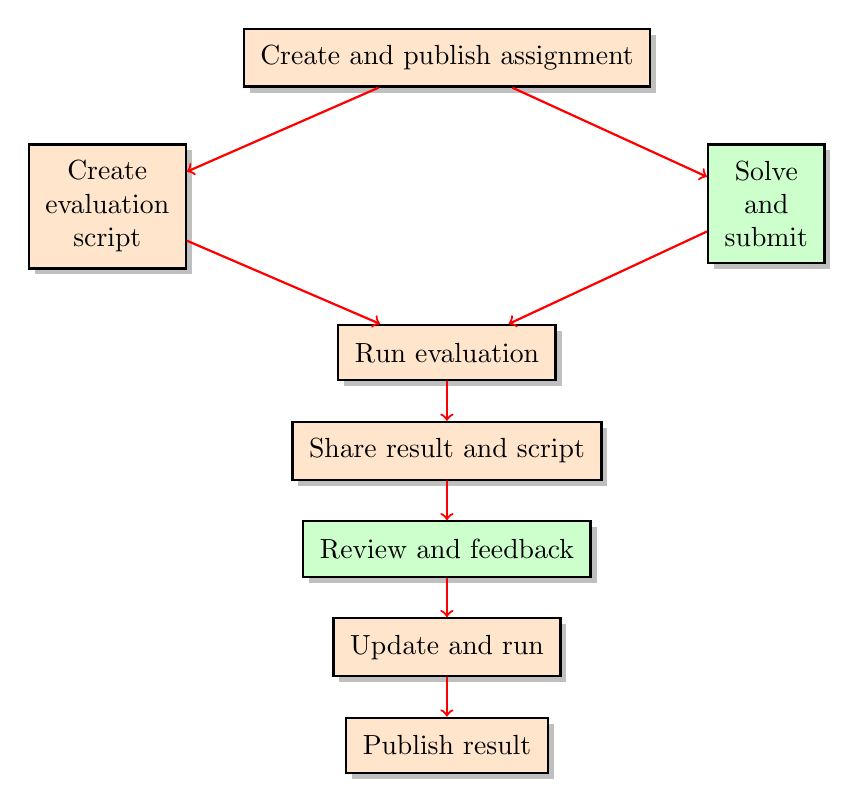
\begin{tikzpicture}
\node[bb, fill=orange!20](1){Create and publish assignment};
\node[bb, fill=orange!20](2)[below left = 1cm of 1]{Create \\ evaluation \\ script};
\node[bb, fill=green!20](3)[below right = 1cm of 1]{Solve \\ and \\ submit};
\node[bb, fill=orange!20](4)[below = 3cm of 1]{Run evaluation};
\node[bb, fill=orange!20](5)[below = 0.5cm of 4]{Share result and script};
\node[bb, fill=green!20](6)[below =  0.5cm of 5]{Review and feedback};
\node[bb, fill=orange!20](7)[below =  0.5cm of 6]{Update and run};
\node[bb, fill=orange!20](8)[below =  0.5cm of 7]{Publish result};

\draw[->, Red, thick](1) -- (2);
\draw[->, Red, thick](1) -- (3);
\draw[->, Red, thick](2) -- (4);
\draw[->, Red, thick](3) -- (4);
\draw[->, Red, thick](4) -- (5);
\draw[->, Red, thick](5) -- (6);
\draw[->, Red, thick](6) -- (7);
\draw[->, Red, thick](7) -- (8);
\end{tikzpicture}
}
\caption{Evaluation workflow}
\label{f:workflow}
\end{figure}

The workflow of our system is shown in fig.~\ref{f:workflow}. The light orange boxes are activities by the instructor and the light green boxes are activities carried out by students. The workflow is congruent with other workflows in the initial part. The instructor creates and publishes the assignment. While the students get busy solving it, the instructor concurrently sets up the evaluation scripts. When the solutions are turned in by the students, the evaluation scripts are run.

A novel aspect of our workflow is that the result of the first run is published along with the evaluation scripts. Students run the scripts on their own end and study the reference solutions. This provides them feedback about their solution as well as with an opportunity to review the reference solutions and provide feedback if needed. We discuss the experiences of following this step in more detail in section~\ref{s:cdebug}.

\subsection{System Architecture}

\begin{figure}

\begin{center}

\resizebox{0.4\textwidth}{!}{
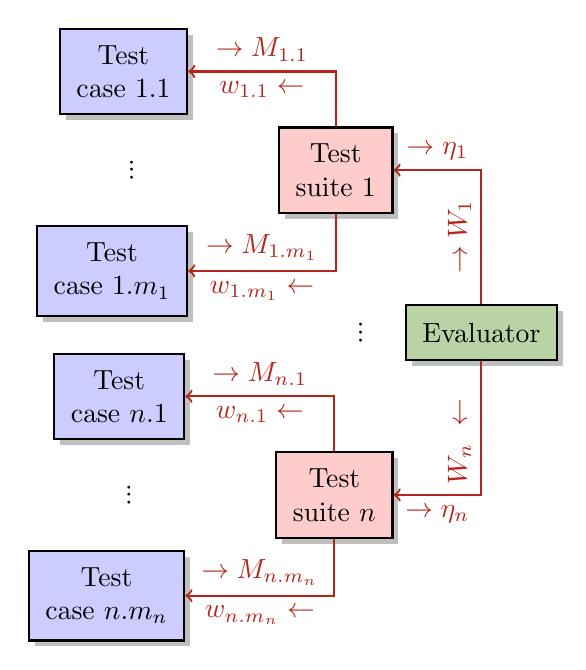
\begin{tikzpicture}
\node[bb](ev){Evaluator};

\node[bb, fill=Red!20, above left= 0.2cm of ev, yshift=1cm](ts1){Test \\ suite 1};
\draw[->, thick, BrickRed](ev) |- node[left, near start] {\rotatebox{90}{$\rightarrow W_1$}} node[above, near end] {$\rightarrow\eta_1$}(ts1);
\node[bb, fill=Red!20, below left= 0.2cm of ev, yshift=-1cm](tsn){Test \\ suite $n$};
\draw[->, thick, BrickRed](ev) |- node[above left] {\rotatebox{90}{$W_n\ \leftarrow $}} node[below, near end]{$\rightarrow\eta_n$}(tsn);

\node[bb, fill=Blue!20, above left= 0.2cm of ts1, xshift=-1cm](tc11){Test \\ case 1.1};
\draw[->, thick, BrickRed](ts1) |- node[below, near end] {$ w_{1.1} \leftarrow$} node[above, near end] {$\rightarrow M_{1.1}$}(tc11);

\node[inv, left= 1.5cm of ts1](dots2){\rotatebox{90}{...}};

\node[bb, fill=Blue!20, below left= 0.2cm of ts1, xshift=-1cm](tc1n){Test \\ case $1.m_1$};
\draw[->, thick, BrickRed](ts1) |- node[below, near end] {$w_{1.m_1} \leftarrow$} node[above, near end] {$\rightarrow M_{1.m_1}$} (tc1n);

\node[bb, fill=Blue!20, above left= 0.2cm of tsn, xshift=-1cm](tcm1){Test \\ case $n.1$};
\draw[->, thick, BrickRed](tsn) |- node[below, near end] {$ w_{n.1} \leftarrow$} node[above, near end] {$\rightarrow M_{n.1}$} (tcm1);

\node[inv, left= 1.5cm of tsn](dots3){\rotatebox{90}{...}};

\node[bb, fill=Blue!20, below left= 0.2cm of tsn, xshift=-1cm](tcmn){Test \\ case $n.m_n$};
\draw[->, thick, BrickRed](tsn) |- node[below, near end] {$w_{n.m_n} \leftarrow$} node[above, near end] {$\rightarrow M_{n.m_n}$} (tcmn);

\node[inv, left= 0.2cm of ev](dots4){\rotatebox{90}{...}};


\end{tikzpicture}
}

\end{center}
\caption{System Architecture}
\label{f:sarch}
\end{figure}

Figure ~\ref{f:sarch} shows the overall architecture under which the evaluation system works.

\subsection{Test cases}
For each programming problem, students typically write one program. Each question often has a number of testable aspects to be checked. In many many cases, these aspects roughly map to individual sub-questions; however, this is not necessary. Typically one, but sometimes more than one, test cases are created to check each of these testable aspects. Each test case is implemented as a function returning 1 on success and 0 on failure along with other relevant information.

\subsection{Test suites}
We would typically have a number of test cases to check a single problem. The number of test cases for question of average size is around 5-10. However, questions with up to 20-25 test cases are not uncommon. These test cases are then bundled into test suites. Hence, one test suite is created corresponding to each programming problem. A test suite computes an overall efficiency $\eta$, which is in the range 0 to 1, indicating the efficiency with which the corresponding problem was solved, corresponding to the problem under question by combining the result of all test cases. $\eta$ is computed as follows:

\begin{equation}
\eta = \frac{\Sigma wM}{\Sigma w}
\end{equation}

where $M$ is 1 or 0 depending on whether the corresponding test case passed or failed, and $w$ is the relative weight or importance of the aspect being tested by the corresponding test case.

\subsection{Evaluator}
All test suites are finally utilised by the central evaluator to compute the marks for the given problem as follows:
\begin{equation}
total = \Sigma \eta W
\end{equation}

where $W$ is the maximum marks allotted to the given problem.

 
\subsection{Implementation}
The evaluation system for a specific assessment is a combination of assessment specific code written by the instructor/TA, and some boilerplate code already provided as a library named \lstinline|evaluate| \footnote{\href{https://github.com/sujitkc/evaluate/}{https://github.com/sujitkc/evaluate/}}. Instructor's main task is to create the individual test cases and organise them within test suites. The \lstinline|evaluate| library provides the glue that puts together this code under the structure shown in fig.~\ref{f:sarch}. Additionally it provides utility scripts useful during the process of evaluation, e.g. preparing marks reports, sending emails, rudimentary plagiarism detection etc. The test case code written by the instructor, nevertheless, typically would run into several hundred lines of code. However, much of it is of repetitive nature. The system assists the instructor by generating stub code for such repetitive parts so that the instructor may focus on the assessment specific code.

In its current form, the system does not automatically design and generate test cases.

\section{Designing Questions}
An important objective of introductory programming courses is to introduce students to basic programming constructs (e.g. branches, loops, functions, recursion, classes and inheritance), and preliminary application of these to solve \emph{very simple} computing problems. These courses stop short of teaching more advanced program design concepts, e.g. data-structure and algorithm design, which are covered in later courses. This results in a fairly regimented nature of what can be asked and how these questions can be answered. The level of abstraction of questions focuses primarily on programming constructs and not on program design. For example, if a question is about implementation of the factorial function, it will mostly be specified if the solution should use iteration or recursion. Note that the objective of such a question would be to test whether the student has understood such programming concepts as loops or recursions, and not to test his/her understanding of the factorial function, which is either assumed to be known or is given in a mathematical form.

Questions designed at a high level of abstraction are desirable because they force the student to model the problem and design a solution. The number of design decisions the student has to take in this process commensurately increases the probability of going wrong or getting stuck. Succeeding in solving such a problem is a good indicator of the student having `got it'. However, not being able to solve such complex design problems is not an indicator that the student has not understood the concepts. In case of failure to solve a complex problem, the problem of analysing the exact reason for failure is often intractable, and totally not worth it.

The above observation leads to the following conclusion: \emph{questions should be designed at a very fine-grained level, without compromising what is being tested.} Having said that, it is a significant challenge to design a question which does indeed test the student's knowledge on the topic in question. An obvious prerequisite to design such a question is a clarity about what is it that the student is supposed to know. Thus, questions should use \textit{learning objectives} as one of the primary references. If a learning objective requires the student to know how to write a for loop in Python, then any question that requires him/her to use for loop will suffice. For example:
\begin{enumerate}
\item Write a program that computes the factorial of a variable \lstinline@x@ which is defined in the beginning of the program. Use a for loop.
\item Write a program that prints "Hello world." ten times. Use a for loop.
\item Write a program that computes and prints the sum of all numbers in a list. Use a for loop.
\end{enumerate}

Note how some of the questions above are constraining the solution space to use only for loop. This is because the primary problem can be solved using other means too, e.g. while loop or recursion.

\section{Designing Test Cases}
From the point of view of test cases, there are a number of types of test cases each catering to a specific testing requirement. We elaborate on this aspect below.

\subsection{Programs with input/output} \label{s:pio}
If the output (into standard output) of a program is what needs to be tested, then the program should be executed and its output should be captured appropriately to be compared against an expected output.

\begin{figure}
\begin{mdframed}[frametitle=Example]
Write a function \lstinline[style=pc]@banner($m$)@ that prints prints the message $m$ decorated with borders. For example, \lstinline[style=pc]@banner("Good Morning!")@ will give:

\begin{lstlisting}[style=oc]
*****************
*_Good Morning!_*
*****************
\end{lstlisting}
\end{mdframed}

(a)

\begin{lstlisting}[style=pc]
@E.evaluate
def eval_1():
  fname = __name__ + "." + sys._getframe()\
          .f_code.co_name
  return E.eval_named_proc_1(fname, driver = \
          "banner_driver.py")
\end{lstlisting}

(b)
\caption{Testing program printing result to standard output}
\label{f:pso}
\end{figure}
The advantage with this kind of test cases is that they are by-and-large agnostic to the internal details of the program being evaluated. Hence, such test cases can be auto-generated to a large extent.

However, due to dependence on input/output (IO), such test cases also tend to be the most fragile: any mistake in the expected input format or the format of output results in the test case failing. Another common source of failure in this kind of test cases is spurious IO code inserted by the student during code, most probably for testing purpose, but later not removed during submission. This form of communication between the submitted program and test harness also puts severe limitations on the complexity or sophistication of the input/output data to/from the program.

Neither is there an easy fix to the fragility of this form of test cases, nor are this kind of test cases entirely avoidable. This is because, in most introductory programming courses, such problems must often be some of the first set of problems solved by the students.

Fig.~\ref{f:pso}(a) shows an example where the program should write the result to the standard output. The test case function shown in Fig.~\ref{f:pso}(b) uses the inbuilt function \lstinline[style=pc]|eval_named_proc_1| of \lstinline[style=pc]|evaluate| library.

\subsection{Programs using/computing values}
Programs using input values from another part of the program computing values which then may get consumed by another part of the program are the next broad category of programs that students get to write. For example:

\begin{figure}
\begin{mdframed}[frametitle=Example]
Write a program to check if a given expression has balanced parentheses. The input string is allowed to contain only three types of brackets: parentheses, i.e. \lstinline[style=pc]@'('@/\lstinline[style=pc]@')'@, curly braces \lstinline[style=pc]@'{'@/\lstinline[style=pc]@'}'@ and square brackets \lstinline[style=pc]@'['@/\lstinline[style=pc]@']'@.

(Hint: Implement a stack in Python using lists)

\end{mdframed}

(a)

\begin{lstlisting}[style=pc]
def eval_program():
  subprocess.call(["rm", "mycode/proginput.py"])
  subprocess.call(["rm", "code/proginput.py"])
  subprocess.call(["cp", "input/proginput.py",
    "mycode/proginput.py"])
  subprocess.call(["cp", "input/proginput.py",
    "code/proginput.py"])
  import code.prog
  import mycode.prog

  if(equals(code.prog.output, mycode.prog.output)):
    return (1, "eval_prog" + ".eval_program")
  else:
    return (0, "eval_prog" +
     ".eval_program: wrong answer")
\end{lstlisting}

(b)
\caption{Testing programs accepting external inputs}
\label{f:pio}
\end{figure}

An example of this type of programming problems is shown in Fig.~\ref{f:pio}(a). In this problem, the student is required to accept the input in the form of a value stored in an input variable. Likewise, the solution program should store its result in an output variable.

The test case, shown in Fig.~\ref{f:pio}(b), has to plug in input (program fragment that supplies input values to the submitted program) and output code (which traps the value generated by the submitted program and checks its correctness) to such programs. Here, the input values are present in input file \texttt{proginput.py}. The answer/result/output of the computation done by the student code is supposed to be stored in a variable named \lstinline[style=pc]|output| whose value is compared against the expected value (generated by the reference code). The advantage here is that the test case is agnostic to the internal details of the program under test, and hence, can by and large be auto-generated.


\subsection{Functions returning value}
The simplest type of test cases are those which test if the output returned by a particular function is correct or not, e.g. whether an implementation of factorial function indeed returns the correct value, or whether the area of a triangle is computed correctly based on its base and height. In most cases, the value returned from a function of this kind is a simple piece of data which can be directly compared with the expected value. In some cases, the equality between actual output and the expected output may not be as straightforward to establish. In such cases, the oracle to test equality should be provided as a parameter to test case.

\begin{figure}
\begin{mdframed}[frametitle=Example]
Write a function \lstinline[style=pc]@product_of_list@ that computes the product of all numbers in a list. For example:
Example:
\begin{lstlisting}[style=pc]
print(product_of_list([1, 2, 3]))
\end{lstlisting}
will print
\begin{lstlisting}[style=oc]
6
\end{lstlisting}
\end{mdframed}

(a)

\begin{lstlisting}[style=pc]
@E.evaluate
def eval_product_of_list_1():
  fname = __name__ + "." + sys._getframe()\
           .f_code.co_name

  from code import Q3 as Sub
  from mycode import evaluate_SOP as Ref

  o = lambda: Sub.product_of_list(t3)
  e = lambda: Ref.product_of_list(t3)
  return E.eval_matfun(fname, o, e)
\end{lstlisting}

(b)
\caption{Testing functions returning value}
\label{f:frv}
\end{figure}

Fig.~\ref{f:frv}(a) shows an example of a problem where a function returns a value as its result. Fig.~\ref{f:frv}(b) shows a test case written in our system to test the function. \lstinline[style=pc]|eval_matfun| is a inbuilt function in \lstinline[style=pc]|evaluate| library.
\subsection{Functions with input/output}
There are function (procedures, to be precise) which depend on/result in \emph{side effects}, e.g. writing into the output console. Such functions should be called and their output (console) should captured appropriately.


\begin{mdframed}[frametitle=Example]
Implement a function that computes the factorial of a number input through standard input and prints out the result on the standard output.
\end{mdframed}

The test cases for such problems are similar to those involving direct input/output (section~\ref*{s:pio}). Hence, these test cases have a similar set of advantages and disadvantages as those. 

\subsection{Questions about Structural Properties}
This form of programming problems strictly do not test the functional properties of a program, but its structural aspects.

\begin{figure}
\begin{mdframed}[frametitle=Example]
Implement function \lstinline[style=pc]@subtract@ using \lstinline[style=pc]@decrement@.
\end{mdframed}

(a)

\begin{lstlisting}[style=pc]
@E.evaluate
def eval_subtract_2():
  fname = __name__ + "." + sys._getframe()\
           .f_code.co_name

  caller = "subtract"
  callee = "decrement"
  if(E.f_calls_g("code/Q2.py", caller, callee)):
    return(1, fname)
  else:
    return(0, fname + " : " + caller + \
        " doesn't call " + callee + ".")
\end{lstlisting}

(b)
\caption{Testing structural properties}
\label{f:ps}
\end{figure}

Fig.~\ref{f:ps}(a) shows an example problem where it is mandated the the function \lstinline[style=pc]|subtract| be implemented using \lstinline[style=pc]|decrement|. This question requires multiple test cases to evaluate, both to test the correctness of the result and to check if \lstinline[style=pc]|subtract| is indeed implemented using \lstinline[style=pc]|decrement|. The latter is checked using the test shown in Fif.~\ref{f:ps}(b). It uses the inbuilt function \lstinline[style=pc]|f_calls_g| of \lstinline[style=pc]|evaluate| library.

We have implemented in \lstinline[style=pc]|evaluate| library a set of function to check some of these commonly checked properties, e.g. \lstinline[style=pc]|f_calls_g| (if a procedure calls another), \lstinline[style=pc]|is_recursive| (if a procedure is recursive), \lstinline[style=pc]|is_inner_function| (if one procedure is an inner function of another), \lstinline[style=pc]|is_subclass| (if a class is a subclass of another) etc.

We wish to reiterate that \lstinline[style=pc]|evaluate| library is the tangible embodiment of the ideas presented in this paper. It can be downloaded and used by anyone who wishes to use the approach presented here.

\section{Experience}

\subsection{The AEPA system}
The AEPA system described in this paper has been used as a part several runs of an introductory programming course (Programming - Python) and an advanced course on Programming Languages (involving functional programming using OCaml) that the author teaches at his university. Though no formal data collection has been made, following are some rough figures:
\begin{enumerate}
\item \textbf{Evaluation scale.} Each run of a course typically has 7-8 programming assignments. Each assignment has 5-10 programming questions, each in turn having 2-5 sub questions. Further, there are two large examinations conducted, each of a scale of a single assignment sheet.
\item \textbf{Program size.} Each question involves at the minimum writing minimum of 2-3 lines of code and maximum of 25-30 lines of code.
\item \textbf{Assessment effort.} The class size is about 150 students. This gives us an estimated 18000-20000 programming questions to be evaluated over the semester. Even with a minute spent manually evaluating each question (which is a conservative estimate), the evaluation effort over the entire semester is about 40 days excluding other non-programmatic assessments (theory, project demos etc.). Considering a semester with about 90-100 working days in it, this amounts to close to nearly half the entire duration of the semester. This is clearly far above what an instructor can afford to spend on evaluating answers. Even if some of this work is offloaded to TAs (which is not an easy thing to do in our circumstances), the high cost of the evaluation process can not be ignored.
\end{enumerate}

Contrary to the manual evaluation, the author has been able to do all corrections automatically with no or very little help from the TAs using the system presented in this paper. The major portion of the effort in this approach goes in designing the questions and test cases. Each assessment instrument (assignment/examination) requires about one day's effort to create the questions and test cases. Automated evaluation requires about 1-2 hours' effort. Detailed evaluation reports get prepared and sent to the students immediately after the evaluation gets done. This significantly shortens the feedback cycle length. Though we do not yet have enough longitudinal data, it is expected that the evaluation effort will drop significantly in future when it gets amortised over all the times an item already added to the item bank is reused.

Following are the achievements of our approach to automated evaluation. Some of these are advantages with respect to platforms like DomJudge:
\begin{enumerate}
\item \textbf{Simple setup.} Our system is based on the policy of having all data on the local machine. This simplifies the setup of the system which is lightweight and local. The boilerplate library code is all in Python. Hence, software requirements are very minimal and light.
\item \textbf{Simple use.} Likewise, the actual evaluation also happens on the local machine of the instructor/TA. No connection to the Internet is required. Of course, a learning management system like \cite{moodle} may be used to facilitate release of the assignment and submissions, but is not essential.
\item \textbf{Language independence.} It is straightforward to use the AEPA system for assignments in a variety of programming languages as the test cases can be designed to be language independent. The system has already been used by us in two flavours: Python and OCaml.
\item \textbf{Data availability.} As the code submitted is not locked inside the database of the system, extracting them for any other purpose is not an issue at all. The code that was submitted for evaluation using our system during our courses have been extensively used by us for our other related research work\cite{10.1145/3412841.3442140}.
\end{enumerate}

\subsection{Crowdsourced Debugging} \label{s:cdebug}
A very interesting aspect of our evaluation process is how we achieve quality assurance for our evaluation scripts. As explained in section~\ref{s:workflow}, all evaluation is done in two steps. In the first step, the instructor creates and executes the test scripts. The output of this round of evaluation, along with the complete evaluation scripts, is shared with the students for review. Students run the scripts on their end and satisfy themselves that the scripts are bug-free, fair and complete. If the students find any bug or other issues, they point it out in an open discussion in LMS. Once the window for feedback closes, the instructor resolves all issues pointed out, and re-runs the scripts. The results thus generated constitute the final marks for the assignments.

The above approach to assure the quality of evaluation scripts has many advantages:
\begin{enumerate}
\item \emph{Transparency:} The transparency achieved by sharing evaluation scripts with students is significantly higher than any other method. Students not only get to see the test inputs but also how they are used to compute the marks. The package shared with the students also includes a reference solution which gets used in the script to compute the expected output. This acts as a model solution for students.
\item \emph{Crowdsourced debugging.} In rare cases, if there are any errors in the scripts, those get uncovered due to the extensive review. The idea of making students debug the scripts turns out to be a very effective pedagogical tool. As marks are at stake, generally  students take the task of reviewing the scripts very seriously. Hence, the review process is very effcient and effective from error discovery perspective.
\item \emph{Teaching by example.} Many students have declared that reading the evaluation script code itself has been a very good learning experience for them. For most students, the scripts code is the first piece of non-trivial software code that they have seen. Many software design principles like modularisation and abstraction are extensively used in the scripts. There are numerous examples of many of the programming techniques and features which are discussed in class (e.g. functional programming, higher order functions, decorators, modules).
\end{enumerate}
\section{Conclusion}
In this paper, we have described a homegrown AEPA system. We have defined an overall architecture of evaluation. We have identified the parts of automated evaluation which are repeatable across assessments; such parts are extracted into boilerplate modules of our system. We have explained the process involved in writing test cases, based on a set of test case types identified here. Our approach, though one among many solutions existing, offers some unique ideas. Firstly, the AEPA system, being a locally installed system, reduces dependence on heavyweight infrastructures like servers and continuous Internet connection. Secondly, the flexible architecture enables checking a wide variety of structural elements as well as functional ones. Finally, involving students in reviewing the test scripts yields unprecedented transparency and learning benefits while bolstering the quality of the scripts themselves.

Our future research has two main aims: one, to make fundamental contributions to the algorithmic issues involved in the AEPA problem; two, to improve the current system to offer better functional and usability features: e.g. web-based/GUI interface, automated test generation, and more fine-grained characterisation of question and test case types. Further, The experiences shared in this paper are based on the our personal experience. A number of other faculty members in our institute have shown interest in using our automated evaluation system. We are currently in the process of helping them adopt this system to their courses.


\bibliography{references}
\bibliographystyle{apalike}

\end{document}
\endinput
%%
%% End of file `sample-sigconf.tex'.
